\documentclass[12pt]{article}
\usepackage[margin=1in]{geometry}
\usepackage{amsmath}
\usepackage{graphicx}

\title{E155 Final Project Status Report: $\mu$Mudd Mark V Debugging and Lab 6 Revision}
\author{Christopher Ferrarin and Kaveh Pezeshki}
\date{14 December 2018}

\begin{document}
	\begin{LARGE}
	\noindent
		E155 
		Final 
		Project 
        Report
		$\mu$Mudd 
		Mark V.1 \\
		Bringup, Redesign
		and 
		Lab 
		6 
		Revision
	\end{LARGE}

	\vspace{0.2cm}
	
	\begin{large}
	Christopher Ferrarin and Kaveh Pezeshki
	
	14 December 2018
	\end{large}
	
	\vspace{5cm}
\begin{abstract}
    The current ENGR155 development platforms, an Altera Cyclone IV on the $\mu$Mudd Mark IV and Raspberry Pi 3, present an unbalanced system. The Raspberry Pi 3 is fast enough to invalidate the need for the Cyclone IV in all situations aside from those requiring precise timing, many I/O pins, or other FPGA-specific features. Our project involves bringup of a $\mu$Mudd redesign that incorporates an ARM MCU, creation of peripheral drivers for the new ARM MCU, and a redesign of Lab 6: Internet of Things. We believe that the new $\mu$Mudd will solve the imbalance between the MCU and FPGA, and allow for final projects more representative of real-world embedded development work.
\end{abstract}
\newpage
\section{Introduction}
    ENGR155 currently uses a Raspberry Pi 3 SoC (System on Chip) and Cyclone IV FPGA as a combined embedded system. Students are expected to work with both devices through the course's labs, and to create a final project that meaningfully implements both the SoC and FPGA. However, this system is unbalanced. The Raspberry Pi 3 uses a modern quad-core SoC, implementing ARM Cortex A-series cores running at 1.2 GHz. It is a device optimized for general computing rather than embedded tasks. The Cyclone IV FPGA, implemented on the in-house $\mu$Mudd development board, is extremely slow in comparison, useful only for timing-critical or I/O-heavy tasks. This projects aims to solve the SoC-FPGA imbalance by bringing up the next-generation $\mu$Mudd Mark V that implements an onboard microcontroller, and reworking critical labs.
    
\subsection{Technical Issues}
    There were three blocking technical issues that prevented the adoption of the $\mu$Mudd Mark V in the course. We aimed to solve these three issues in our project:
    
    \begin{enumerate}
        \item The $\mu$Mudd Mark V, as provided at the start of the project, had a nonfunctional MCU. We needed to identify the blocking bugs in the new PCB layout and MCU implementation, and implement fixes to these issues in the schematics and layout for the board.
        \item The ARM MCU implemented on the $\mu$Mudd Mark V uses a different peripheral set and memory map compared to the Broadcom SoC on the Raspberry Pi 3. We needed to write an equivalent to easyPIO.h, the peripheral driver header file for the Raspberry Pi 3, for the new ARM MCU.
        \item Lab 6: Internet of Things, requires an HTTP web server implemented on the Raspberry Pi 3. It is infeasible for students to write an HTTP web server from first principles on a bare ARM MCU, so we needed to redesign Lab 6 to better fit the new $\mu$Mudd while retaining internet access, wireless communication, or another component of the general IoT device.
    \end{enumerate}
\subsection{Board Design}
    Last year, a team of students designed a new $\mu$Mudd board to rebalance the MCU (microcontroller) or SoC  and FPGA platform. They could not upgrade the FPGA, as the current Cyclone IV is the highest-end FPGA available in a hand-solderable form factor as required by the $\mu$Mudd. Instead, they moved from the Raspberry Pi 3 SoC to an Atmel SAM4S series MCU on the $\mu$Mudd, which implements a single Cortex M4 core, benchmarking near 38 times slower than the Raspberry Pi 3 in CoreMark [1][2], and a peripheral set much more well-suited to mixed-signal embedded applications. This combination of MCU and FPGA is much more well-balanced, and allows for meaningful use of the FPGA as a compute accelerator. The student team also implemented new features to the board, including an external test board which checks that the MCU and FPGA are operational before assembly in Lab 1. Experience from ENGR085 will carry to this new board, as Keil can be used for device programming.
    
    Upon starting this project, we were presented with a nonfunctional version of the next-generation ENGR155 board: the $\mu$Mudd Mark V, as well as a set of schematics implementing proposed fixes to the board. While design flaws in the board prevented the MCU from executing code, the board incorporated all of the main features expected from the $\mu$Mudd Mark V. The combined FPGA / MCU system is illustrated in Figure \ref{pcb_block}.
    
    \begin{figure}[h]
        \label{pcb_block}
        \begin{center}
            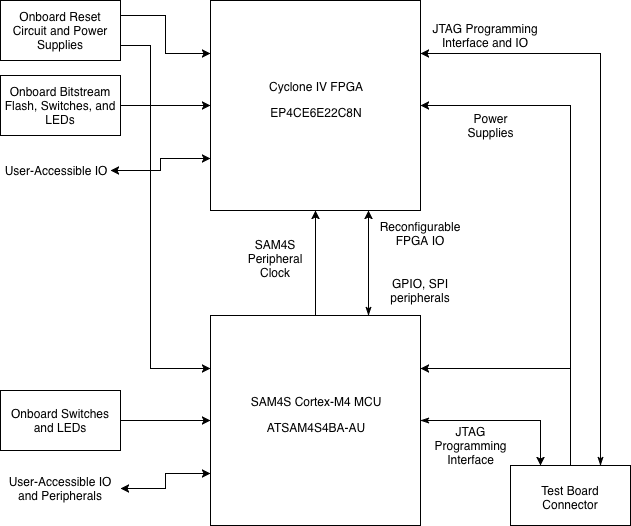
\includegraphics[width=10cm]{blockdiagrampcb.png}
            \caption{Block Diagram of the Redesigned $\mu$Mudd}
        \end{center}
    \end{figure}
    
\subsection{Lab 6 Design}
    While most of the labs implementing the Raspberry Pi 3 could be easily altered to instead use the SAM4S microcontroller, Lab 6 demanded a redesign. Currently, Lab 6 tasks students with developing a system which provides control over LEDs on the Raspberry Pi 3 GPIO and fetches current light intensity as measured by a phototransistor and SPI ADC. This information and control capability must be accessible via a webpage hosted on the system.
    
    The Raspberry Pi 3, with its Linux (Raspbian) operating system, had a simple means of hosting an HTML web server in the form of Apache. On the other hand, our microcontroller did not have an operating system at all, and so we sought to retain the learning goals and basic framework of the current Lab 6 while modifying it to be compatible with the SAM4S. Our proposed implementation used an ESP8266 and a WiFi-enabled microcontroller, to host an HTTP webpage as  in the current version of Lab 6, as well as adding an SPI pressure and temperature sensor. The block diagram in Figure \ref{lab6_wifi_block} illustrates this redesign of Lab 6.

    \begin{figure}[h]
        \label{lab6_wifi_block}
        \begin{center}
            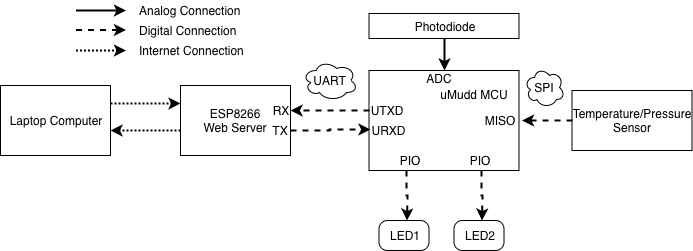
\includegraphics[width=12cm]{blockdiagramwifi.png}
            \caption{Block Diagram of the Lab 6 Proposal}
        \end{center}
    \end{figure}    
    
    
    
\subsection{Device Driver Design}
    In the ENGR155 labs, a core skill students gain is the ability to read the datasheet of a new microcontroller and build up basic functionality for a peripheral. Still, in later labs and in the final project, it is convenient to provide a device driver so that more complicated, higher-level designs can be implemented without the need to spend additional time on low-level peripheral work. With the replacement of the Raspberry Pi 3 with a microcontroller came the need to develop a new device driver for the SAM4S. While many exist due to the prevalence of the ARM Cortex-M series, we sought to develop one simple enough for students to understand while robust enough to handle most of the functionality students might use in their final project. This device driver would also be instrumental in our board bringup efforts to help verify functionality of various peripherals and components of the microcontroller as well as in our Lab 6 redesign to create a working prototype.


\section{Implementation and Debug Details}
\subsection{Board Design}

Our initial tasks in the project were to determine the cause of the MCU failures in the $\mu$Mudd Mark V and implement fixes to these bugs in the schematic and layout of the board. 

\subsubsection{$\mu$Mudd Mark V Debug}

After initial testing of the $\mu$Mudd Mark V, we noticed unstable MCU behavior. We were only occasionally able to program the SAM4S, and in the cases where our programmer reported a successful program flash, we were unable to enter the debugger, and the MCU would not execute the program outside of the debugger. 

Further investigation revealed that, in the cases where the programmer indicated a successful program flash, the microcontroller program memory remained initialized to all 1s. This can be observed in Figure 3. 

    \begin{figure}[h]
        \label{deadmemory}
        \begin{center}
            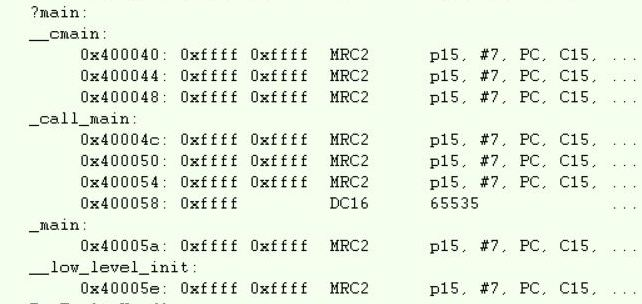
\includegraphics[width=8cm]{deadmemory.JPG}
            \caption{The SAM4S main function program memory after a program flash}
        \end{center}
    \end{figure}
    
We realized that this issue was caused by two bugs in the current PCB design: a wiring error with the flash erase pin on the microcontroller, and potential instability due to to the current microcontroller power supply. 

The largest problem with the current $\mu$Mudd design lies in the MCU ERASE pin, which re-initializes the onboard flash and resets the processor. The ERASE pin can also serve as general-purpose I/O after configuration [3].

On boot, ERASE must be held low to prevent flash erase and re-initialization of the processor. On the current $\mu$Mudd, ERASE was tied to a general I/O pin on the Cyclone IV FPGA. The connection can be seen in the schematic in Figure 4.

\begin{figure}[h]
    \label{eraseerror}
    \begin{center}
    	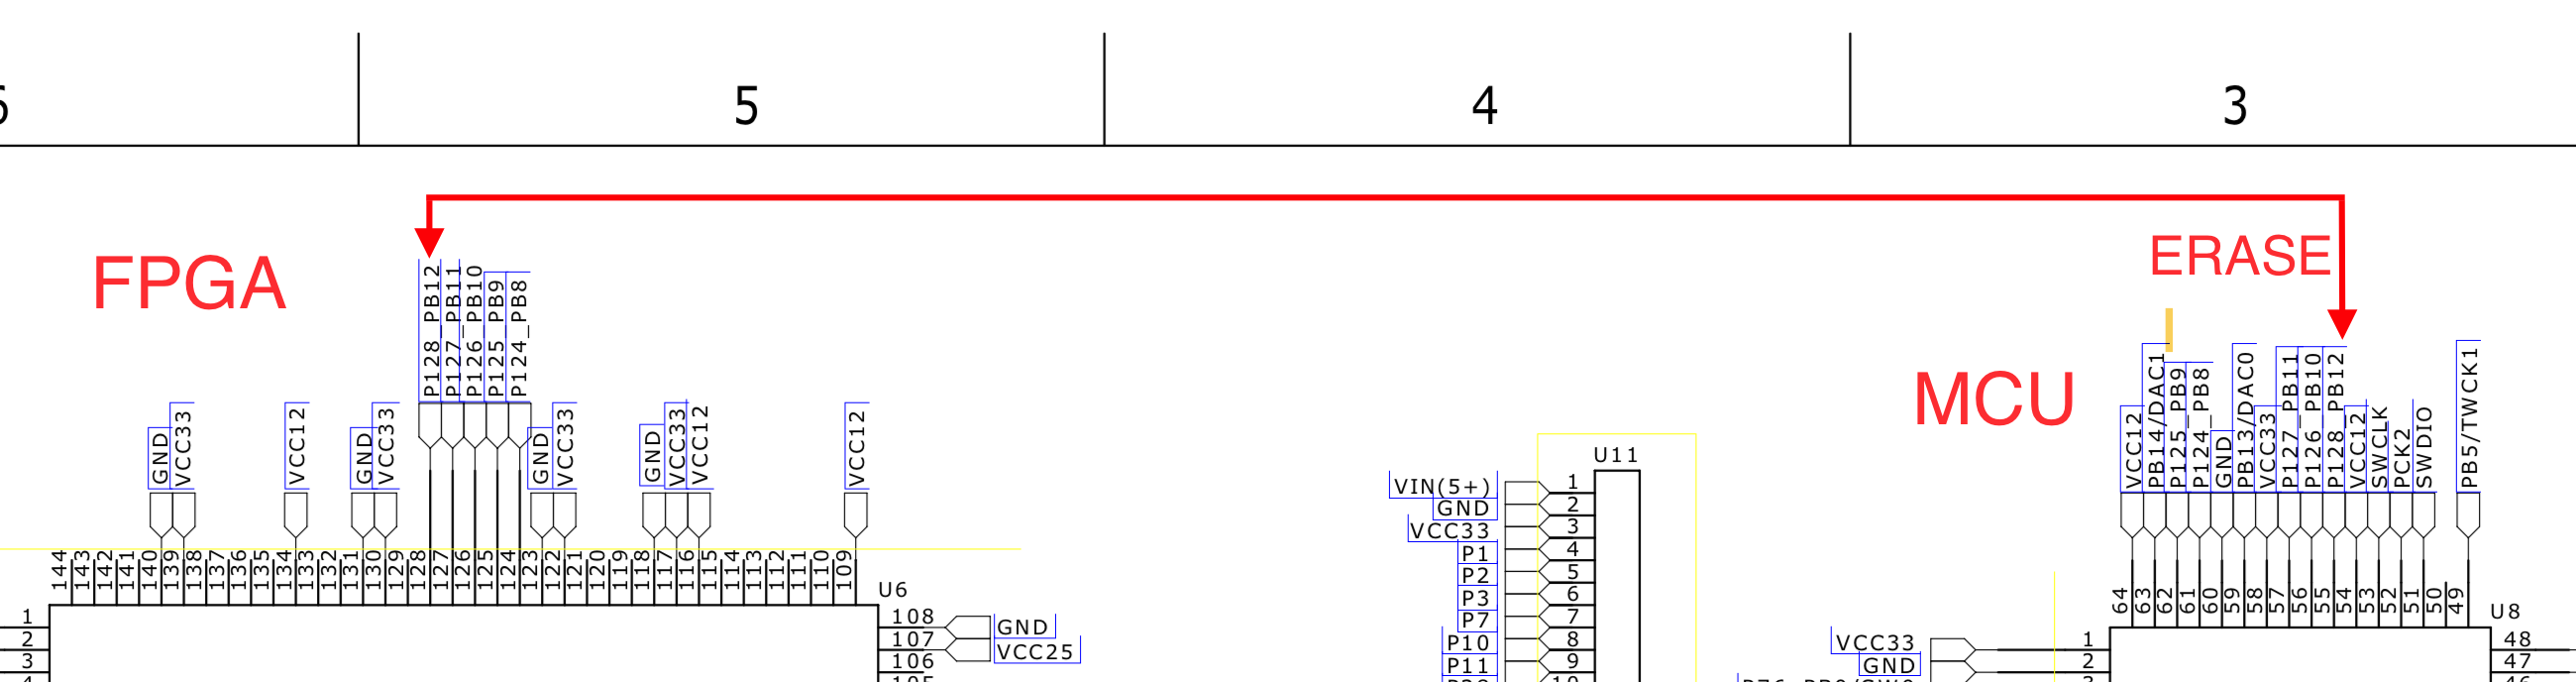
\includegraphics[width=16cm]{erase_error.png}
    	\caption{The marked connection ties ERASE on the MCU to pin 128 on the FPGA}
    \end{center}
\end{figure}

The ERASE pin contains a 100-k$\Omega$ pull-down resistor [3].An unconfigured Cyclone IV I/O pin contains a 25-k$\Omega$ pull-up resistor [4]. This creates a voltage divider circuit as shown in Figure 5. This provides a predicted voltage of 2.64V on the MCU ERASE pin, close to the 2.86V we observed. This is a high logic level which prevented FPGA programming. After correcting this issue by manually breaking the ERASE pin trace, we were able to program and execute code on the $\mu$Mudd.

\begin{figure}[h]
    \label{eraseerrorschematic}
    \begin{center}
    	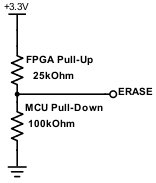
\includegraphics[width=5cm]{resistor_divider.png}
    	\caption{Voltage divider producing a high logic level on the MCU ERASE pin}
    \end{center}
\end{figure}

The second issue with the microcontroller implementation lies in its power supply configuration. The MCU requires a 3.3V and 1.2V power supply. It can be powered via one 3.3V supply, and use an internal regulator to generate 1.2V, or it can be powered with an external 3.3V and a 1.2V supply. On the $\mu$Mudd Mark V, discrete 3.3V and 1.2V regulators power the FPGA and MCU. This dual-regulator design of the current board can introduce microcontroller boot issues if timing is not correct, with proper timing illustrated in Figure 6.

\begin{figure}[h]
    \label{vddtiming}
	\begin{center}
	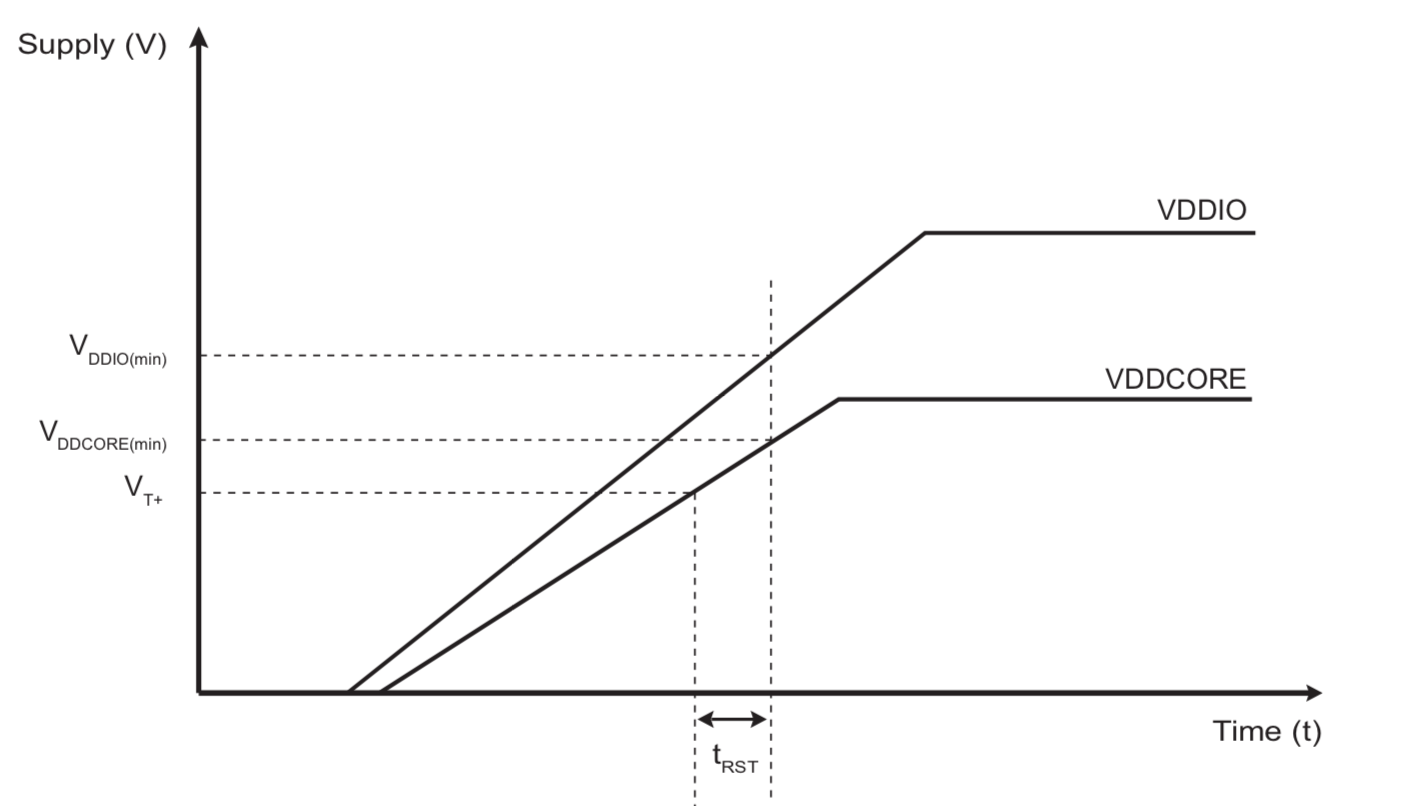
\includegraphics[width=11cm]{power_timing.png}
	\caption{Timing requirements for the 1.2V (VDDCORE) and 3.3V (VDDIO) supplies\footnote{SAM4S Series Datasheet p27}}	
	\end{center}
\end{figure}

We believe that these potential timing errors can cause system instability, as we observed an unresponsive MCU after boot that could only be solved with a full erase and reset.

\subsubsection{$\mu$Mudd Mark V Redesign}

We therefore began a PCB redesign to solve these issue. We incorporated the following changes:

\begin{enumerate}
    \item We tied the ERASE line to a separate pushbutton on the PCB. The FPGA can no longer erase the MCU flash.
    \item We moved MCU core and PLL power supplies to the onboard regulator, with an associated RLC filtering circuit as suggested by the manufacturer [5].
    \item We re-routed the JTAG interface to a smaller connector compatible with the common J-Link EDU Mini ARM programmer [6].
    \item We re-positioned components on the board to allow for easier assembly, as well as for easier button and LED access.
    \item We added via shielding on the MCU to FPGA clock line.
    \item We propagated the above changes to the Lab 1 test board.
\end{enumerate}

The $\mu$Mudd and test board PCBs pass all design tool and manufacturer DFM and DRC checks, and are ready for manufacture at Advanced Circuits. Schematics, layout, and a BoM for the $\mu$Mudd and test board are available in appendices A and B.

\subsection{Lab 6 Design}
The current version of Lab 6 relies on an HTTP webpage hosted by Apache on the Raspberry Pi 3. As the new ENGR155 embedded system no longer runs Linux, we do not have access to common web hosting tools. However, we wanted to maintain a similar feature list to the current Lab 6. In the revised lab, students will have to implement the following:

\begin{enumerate}
    \item A voltage divider circuit to generate voltage proportional to ambient light intensity with a LPT2023 phototransistor
    \item SPI device drivers and support for the BMP280 pressure and temperature sensor
    \item GPIO device drivers to control the state of an two LEDs
    \item A basic web page that provides access to current pressure, humidity, and light intensity, as well as LED on/off buttons 
\end{enumerate}

Students will be provided with code examples for interfacing with the ADC peripheral on the microcontroller, for UART communication, for controlling the state of a single LED, and for hosting a basic HTTP webpage with dynamic data.

This retains the lab objectives of learning basic IoT and web design and of gaining more experience implementing peripherals and sensors from their datasheets. A rewritten lab manual for Lab 6 is available in Appendix 3.

\subsubsection{HTTP Webpage Hosting}

It is a non-trivial task for the $\mu$Mudd board alone to host an HTTP webpage. This would require implementation of a TCP/IP stack, of the HTTP server protocol, and the physical addition of an interface able to connect the $\mu$Mudd to a router. Instead of attempting this implementation, we decided to use an external off-the-shelf platform capable of TCP/IP networking and WiFi. 

In particular, we decided to use an ESP8266 [7], implemented on a NodeMCU ESP-12E [8], as a replacement for the Apache web server. The ESP8266 is a microcontroller platform that implements WiFi and a TCP/IP stack on an RTOS (real-time operating system). This allows the ESP8266 to host or connect to WiFi networks, as well as to act as a client or server in HTTP transactions.

We did not want to require students to implement the webpage hosting backend, as we believed this would increase lab workload to an unacceptable level. The ESP8266 therefore serves as a `black box' peripheral to the $\mu$Mudd, accessible over UART. The student has the ability to reprogram the ESP8266, and will be provided with reference code in which they can specify network connections and IP addresses, as well as providing additional configurability. The ESP8266 also prints debug and status messages on a serial connection over a MicroUSB connector.

On boot, the ESP8266 connects to a network predefined by the user, hosts a WiFi access point, and starts a HTTP server. It then requests a webpage to display from the $\mu$Mudd. Having received a webpage, the server is now ready to handle a HTTP client. 

After the user interacts with or refreshes a webpage, the ESP8266 needs to return the client request to the $\mu$Mudd. A request - response transaction between the ESP8266 and $\mu$Mudd can take upwards of a half-second for a webpage of any reasonable size. This delay led to hangs and crashes in the client browser. We therefore implemented a HTTP server hosting and webpage request - responses with the $\mu$Mudd as semi-independent processes. A new webpage will be requested from the $\mu$Mudd only under the following conditions:

\begin{enumerate}
    \item The user has reloaded or interacted with the webpage since the webpage was last reloaded from the $\mu$Mudd
    \item At least 10 seconds have passed since the last request-response communication from the $\mu$Mudd
\end{enumerate}

The ESP8266-$\mu$Mudd protocol is as follows:

\begin{enumerate}
    \item When requesting a webpage from the $\mu$Mudd, the ESP will transmit an abbreviated URL of the last webpage requested by an HTTP client. For example, if the ESP8266 had an IP address of 192.168.1.2, and the user requested the page http://192.168.1.2/ledon, the ESP8266 would transmit the string ``$<$ledon$>$".
    \item The $\mu$Mudd is then responsible for parsing this abbreviated URL, performing any required actions, and then returning an HTML webpage. The ESP8266 will accept a webpage only if it begins with the string ``$<$!DOCTYPE html$><$html$>$" and ends with the string ``$<$/html$>$"
\end{enumerate}

This restricts users to webpage interaction based on redirects, and leads to a time lag between user action on the webpage and the $\mu$Mudd response. However, this behavior is superficially sufficient for Lab 6. Code for the ESP8266 `black box' peripheral is available in appendix 4. 

\subsubsection{Demo Code}

We have designed a demo webpage to provide students with an example of an IoT device. The demo implements the following features:

\begin{enumerate}
    \item A status LED on pin PA18 which illuminates when a webpage is transmitted over UART
    \item A user-controllable LED on pin PA17
    \item Reading from ADC channel 2 on pin AD2
    \item An ESP8266 interface which hosts a webpage which displays the voltage on AD2, and provides buttons to turn the user-controllable LED on and off
\end{enumerate}

We have demonstrated this lab on the Olimex SAM3-P256 development board as a temporary replacement for the revised $\mu$Mudd Mark V. While the SAM3-P256 implements a SAM3S-series MCU rather than a SAM4S-series MCU, the two chips share identical base instruction sets, peripheral sets, and peripheral memory maps. The schematic for our demo is available in Figure \ref{lab6schematic}, and code for the demo is available in appendix 5. 

\begin{figure}[h]
    \label{lab6schematic}
	\begin{center}
	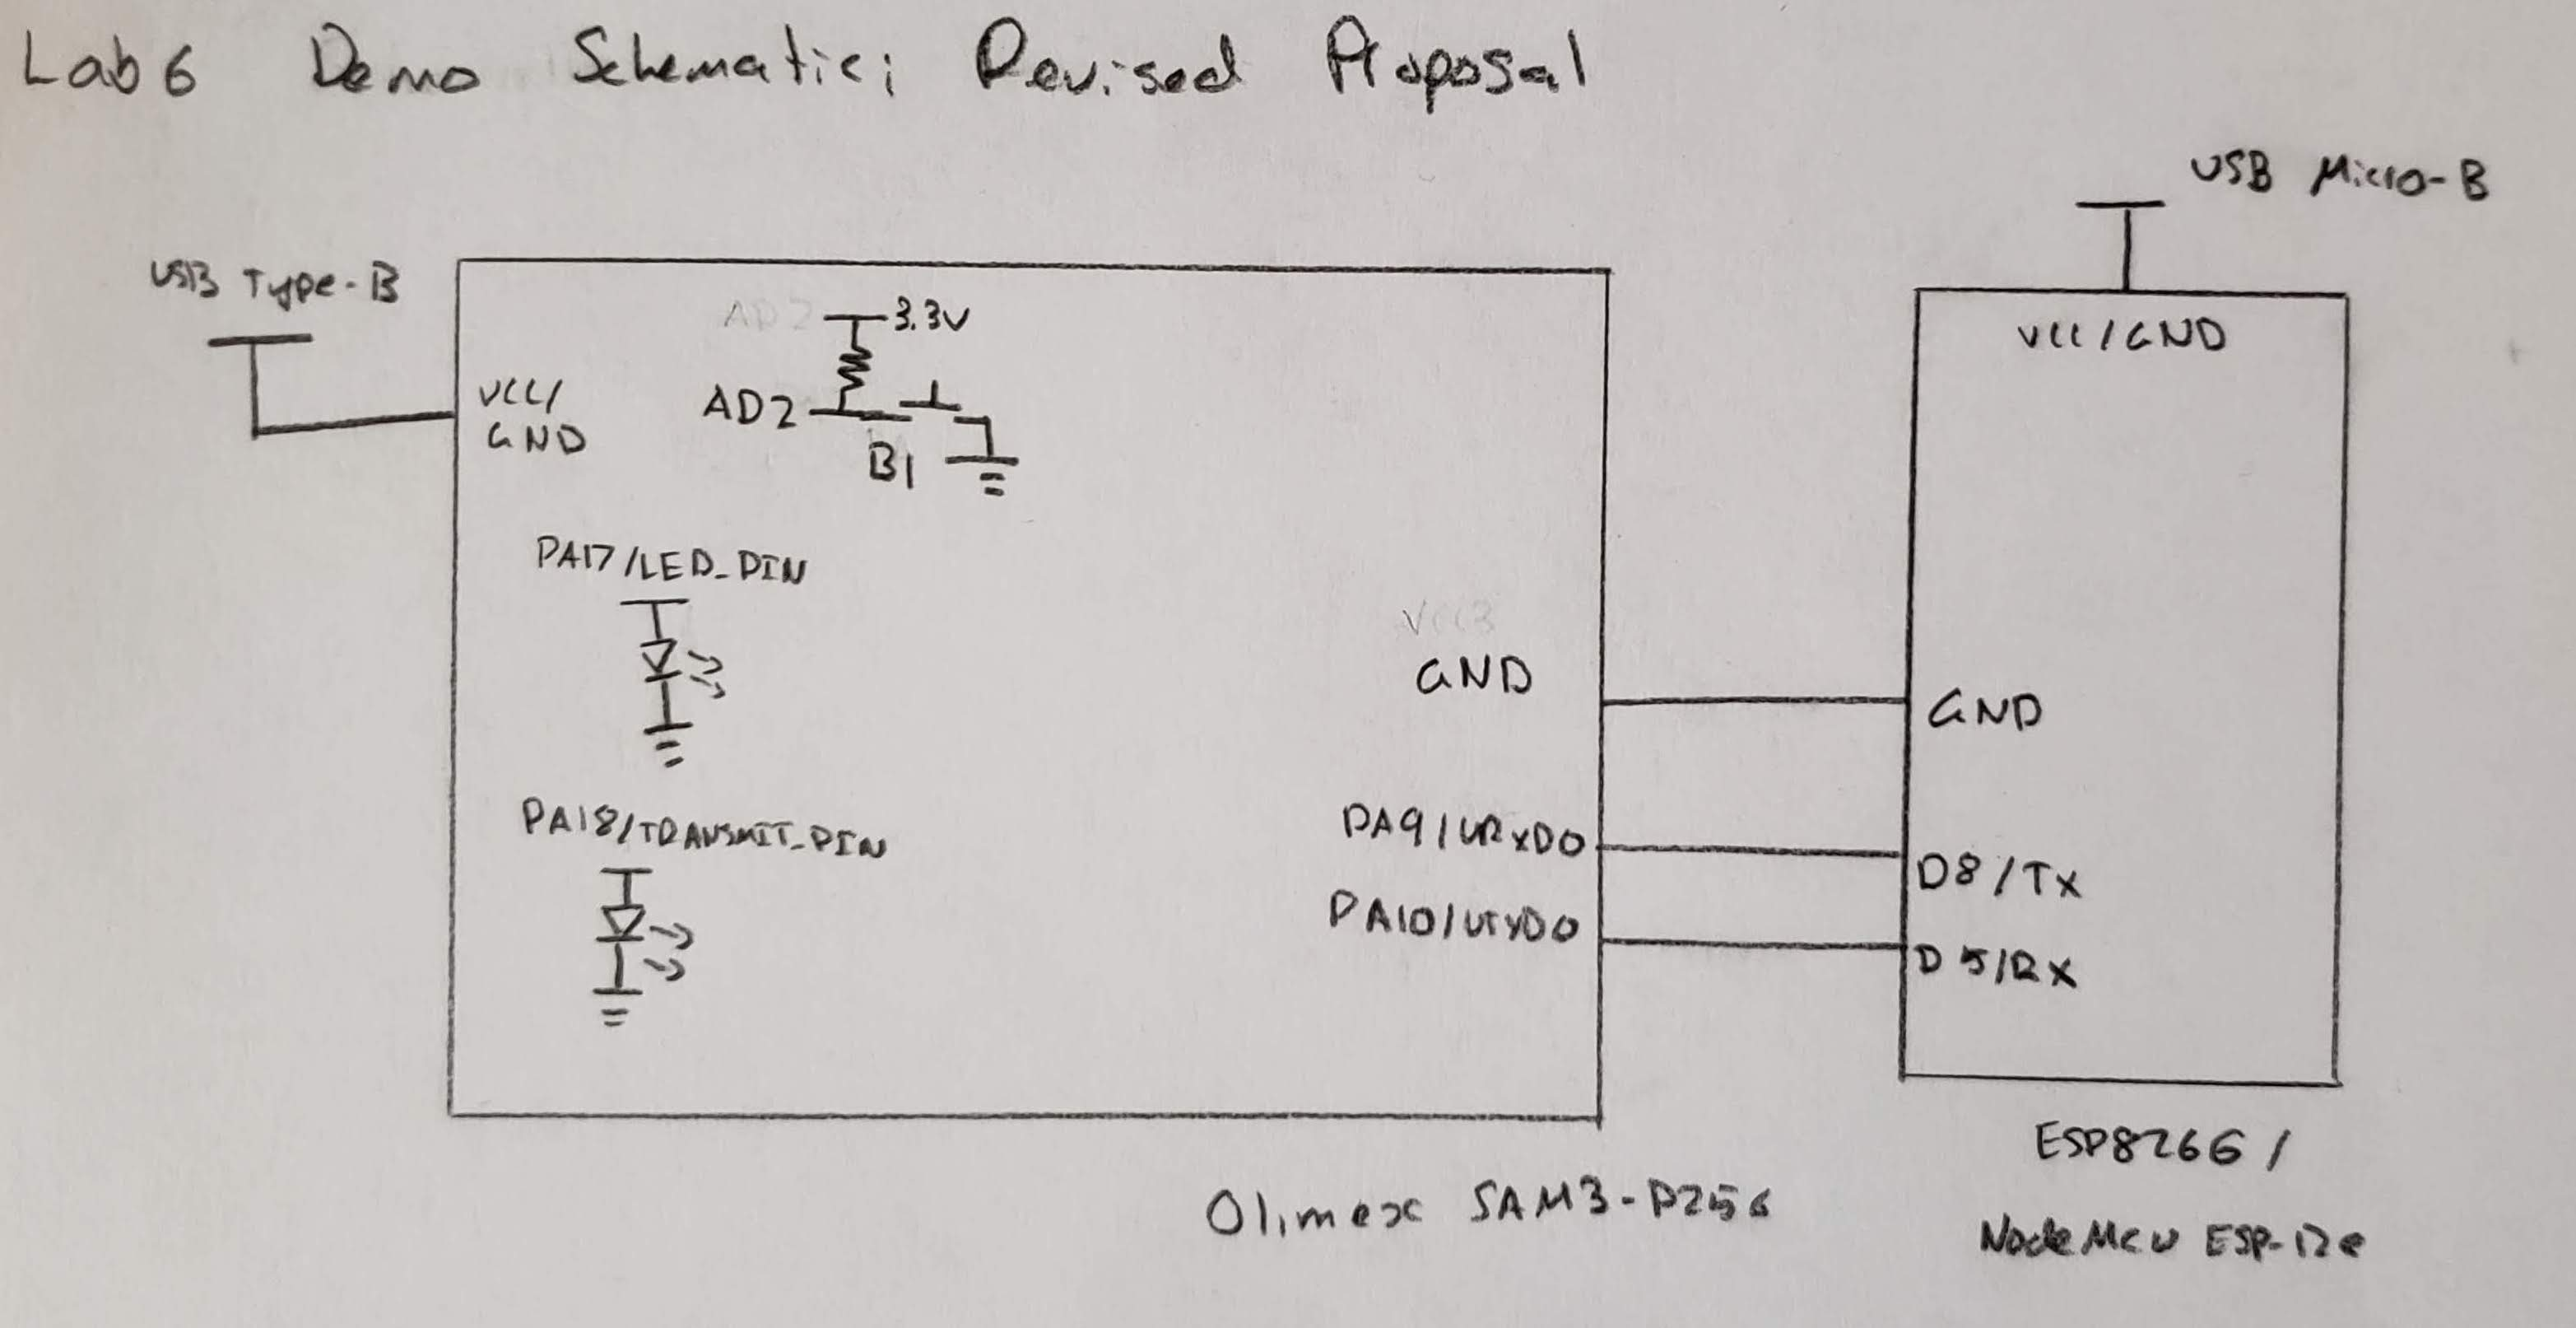
\includegraphics[width=11cm]{lab6_schematic.jpg}
	\caption{Lab 6 Demo Schematic. Note that the circuits implemented in the box to the left are pre-existing peripherals on the Olimex SAM3-P256}	
	\end{center}
\end{figure}

\subsection{Device Driver Design}
    The SAM4S device driver provides minimal working support for the following peripherals:
    \begin{itemize}
        \item PMC (Power Management Controller): For clock multiplexing to peripherals and controlling programmable clocks.
        \item PIO (Parallel Input/Output Controller): For peripheral function pin multiplexing and reading and writing digital values from pins. Both ports (PIOA and PIOB) are supported.
        \item TC (Timer Counter): For system delays and counting and triggering at various clock speeds. Both channels (TC0 and TC1) are supported. Since this peripheral will mostly be used to generate delays, we have provided code that allows students to ignore any other functionality of the Timer Counter in order to simply delay the system, while other low-level code exists if they desire this additional functionality.
        \item SPI (Serial Peripheral Interface): For serial communication with external devices that support SPI.
        \item UART (Universal Asynchronous Receiver-Transmitter): For serial communication with external devices that support UART.
        \item PWM (Pulse Width Modulation Controller): For generating square waves of various frequencies and duty cycles. All four channels (PWM0 - PWM3) are supported.
        \item ADC (Analog-to-Digital Converter): For reading analog voltages.
        \item RTC (Real Time Clock): For automatic tracking of the time and date.
    \end{itemize}
 
    We believe that this set of peripherals will allow students to tackle the majority of tasks they might encounter in later labs and in the final project, while not being so large as to be unwieldy and confusing.
    
    One guiding principle behind our device driver design was organization. We achieved this in three main ways: 
    \begin{enumerate}
        \item We split up the device driver into multiple, independent header files.
        \item We used naming conventions for registers, functions, and definitions that were consistent across peripherals.
        \item We defined all registers and bits using a hierarchy of named structs.
    \end{enumerate}
    
    Dividing the over 1500 lines of code for the device driver into multiple header files has a number of advantages over the previous single easyPIO.h file that was used previously. First, it allows students to more quickly find what they are looking for. For example, if a student wishes to find what inputs the pioPinMode() function can take, rather than searching through a large block of code, they can simply open the SAM4S4B\_pio.h header file and look in the "PIO Functions" block of code. This organizational system also delegates all definitions that the user would be likely to change to the SAM4S4B\_sys.h header file, since it can be difficult to look through a large device driver and deduce which definitions a user can change without breaking a fundamental function. Finally, this system is more efficient; although this is unlikely to be a major problem, compiling and storing a large header file in a microcontroller every time it is reprogrammed can be slow and inefficient. This way, students need only include in #include preprocessor directives those header files for peripherals they are actively using, cutting down on compile time and memory requirements.
    
    Naming conventions for definitions, registers, and functions alike further helps keep the device driver simple and easy to read. Although this makes the code somewhat more verbose, we decided to begin each definition name, register name, and function name of every peripheral with a prefix of that peripheral's name. For example, for the PIO peripheral, a definition might be named PIO\_PA13, a register might be named PIO\_PER, and a function might be named pioInit().
    
    The final change may well be the most significant. In ENGR155, students are taught how to interact with special function registers on the lowest level possible: creating pointers to specific words in memory and then writing or reading bits or fields using bitwise "and" and "or" assign operators and bit shifts. While this provides students a fundamental understanding of the effect of their code on hardware, such code is almost impossible to read without the help of a datasheet, and even then can take a copious amount of time. To improve this aspect of the device driver, we defined every bit, register, and register block with the following hierarchy:

    \begin{figure}[h]
        \label{headerChart}
	    \begin{center}
	        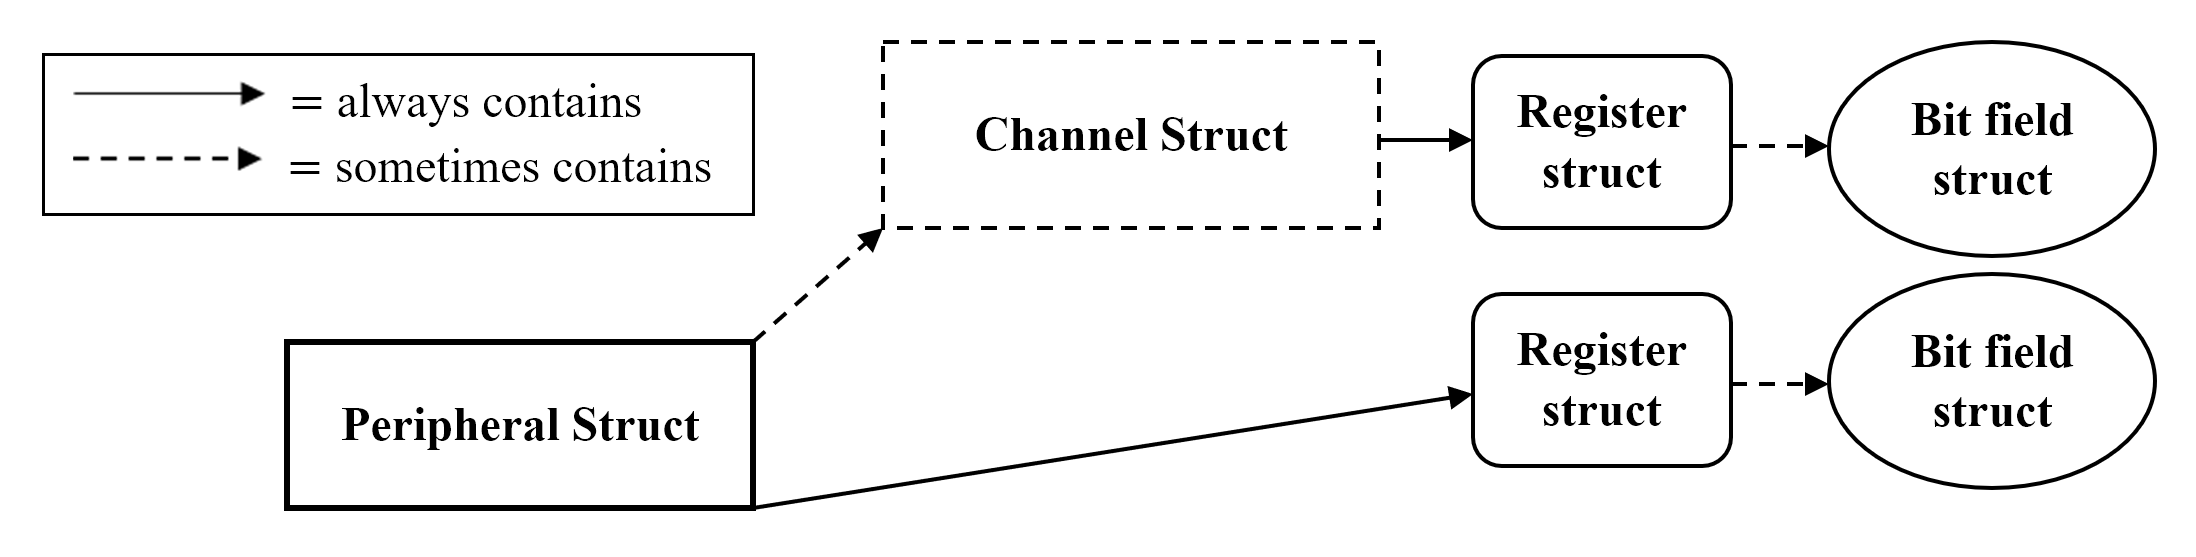
\includegraphics[width=14cm]{headerFileOrganization.png}
	        \caption{Hierarchy of structs used to organize register definitions in the SAM4S device driver.}	
	    \end{center}
    \end{figure}

    In addition, we defined a pointer to every peripheral struct, meaning that students do not need to interact with addresses of words or bit locations within words at all; rather, they interact with the names of registers and bits, which is much more intuitive and readable. Finally, using dot and dereference operators to move down the struct hierarchy results in overall cleaner code than direct low-level operations on words.
    
    Code for the peripheral drivers is available in Appendix F.


\section{Results and Discussion}
% General results for the entire project
Our proposal deliverables were, given verbatim from our proposal:

\begin{enumerate}
    \item Identify blocking bugs in the $\mu$Mudd which completely prevent MCU programming and operation
    \item Determining and implementing a solution to the above bugs. This solution may take several forms, as described below (not restated here)
    \item Reworking Lab 6 with instructor guidance to fit the new $\mu$Mudd MCU
\end{enumerate}

We have successfully completed these tasks. In response to the first two tasks, we have created a revised set of PCBs which solve the MCU programming and program execution issues, as well as providing general quality-of-life improvements. In response to the third task, we have created a revised Lab 6 that retains all IoT elements while providing a meaningful role for the $\mu$Mudd.

Our initial stretch goals of testing labs 4,5, and 7 transitioned into creation of extensive peripheral drivers for the $\mu$Mudd. We believe that this is a more valuable product than purely testing the other microcontroller-related labs, as it provides a framework that vastly simplifies any further lab testing or development. 

Despite this progress, the new $\mu$Mudd and Lab 6 are not yet adequately polished for release into the next session of ENGR155. We would in particular like to improve our ESP8266 web server to eliminate the 10 second maximum delay between client interaction with the webpage and microcontroller response. We plan to implement and test all other labs, rewrite lab manuals, and thoroughly test the revised $\mu$Mudd Mark V over the upcoming semester.


\section{Budget and BOM}

\begin{center}
	\begin{tabular}{llll}
	Item Name & Item Description & Vendor & Item Cost \\
	\hline
	SAM3-P256 & SAM3S Development Board & Olimex & \$31.09 \\
	Ailavi JTAG & JTAG-SWD Adapter & Amazon & \$8.99  \\
	GikFun EK1199 & JTAG-SWD Adapter & Amazon & \$7.66 \\
	J-Link EDU Mini & JTAG Debugger & Adafruit & \$19.95 \\
	ESP8266  & Web Server Module & Amazon & \$5.49 \\
	& & & \\
	Total Budget & & & \$422.19
	\end{tabular}

\end{center}

\begin{thebibliography}{999}
    \bibitem{1}
        Benchmark 2758: Broadcom BCM2837 / Raspberry Pi 3. (2018). 
        Retrieved December 13, 2018, from https://www.eembc.org/benchmark/reports/benchreport.php?
        suite=CORE&bench\_scores=2758
    \bibitem{2}
        Atmel's SAM4S Clinches Highest CoreMark/MHz scores. (2013, June 27). Retrieved December 13, 2018, from https://atmelcorporation.wordpress.com/2013/06/24/atmels-sam4s-clinches-highest-coremarkmhz-scores/
    \bibitem{3}
        “SAM4S Series: SMART ARM-Based Flash MCU Datasheet.”
        Atmel Corporation, San Jose, CA, 2015.
    \bibitem{4}
        Cyclone IV Device Handbook, Volume 1 [PDF].
        (2016, December).
        San Jose, CA: Altera Corporation.
    \bibitem{5}
        Application Note AT03463: SAM4S Schematic Checklist [PDF].
        (2015).
        San Jose, CA: Atmel Corporation.
    \bibitem{6}
        J-Link EDU Mini.
        (2018). 
        Retrieved December 13, 2018, from https://www.segger.com/products/debug-probes/j-link/models/j-link-edu-mini/
    \bibitem{7}
        ESP8266.
        (2018).
        Retrieved December 13, 2018, from https://www.espressif.com/products/hardware/esp8266ex/overview/
    \bibitem{8}
        NodeMCU Documentation.
        (2018, September).
        Retrieved December 13, 2018, from https://nodemcu.readthedocs.io/en/master/
\end{thebibliography}

\newpage
\section*{Appendix A: $\mu$Mudd Schematic and Layout}
\clearpage
\section*{Appendix B: Test Board Schematic and Layout}
\clearpage
\section*{Appendix C: Revised Lab 6 Lab Manual}
\clearpage
\section*{Appendix D: ESP8266 `Black Box' Peripheral Code}
\clearpage
\section*{Appendix E: Lab 6 Demo Code}
\clearpage
\section*{Appendix F: Peripheral Driver Code}
\clearpage

\end{document}
